\documentclass[12pt,twoside,a4paper]{article}
\usepackage[a4paper,width=150mm,top=25mm,bottom=25mm,bindingoffset=6mm]{geometry}

\usepackage[utf8x]{inputenc}
\usepackage[slovak]{babel}
\usepackage{palatino,verbatim}

% Balicek pre priamu rec - \say
\usepackage{dirtytalk}

% Obrazky
\usepackage{graphicx}
\graphicspath{ {obr/} }

% Cislovanie obrazkov a tabuliek
\usepackage{chngcntr}
%Cisluj obrazky nezavisle od cisla kapitol/podkapitol
%\counterwithout{figure}{subsection}
%\counterwithout{table}{subsection}

%Uloz obrazok tam, kde je deklarovany
%\usepackage[subsection]{placeins}

\newcommand\sktxt[1]{\foreignlanguage{slovak}{#1}}

\begin{document}
\pagenumbering{arabic}

\section*{Multi-area OSPF}
\subsection*{Topológia}
\paragraph{}
Budeme konfigurovať Multi-area OSPF, ktorá je znázornená na obrázku ~\ref{fig:multiarea_ospf_topo}.

\begin{figure}[!htb]
\centering
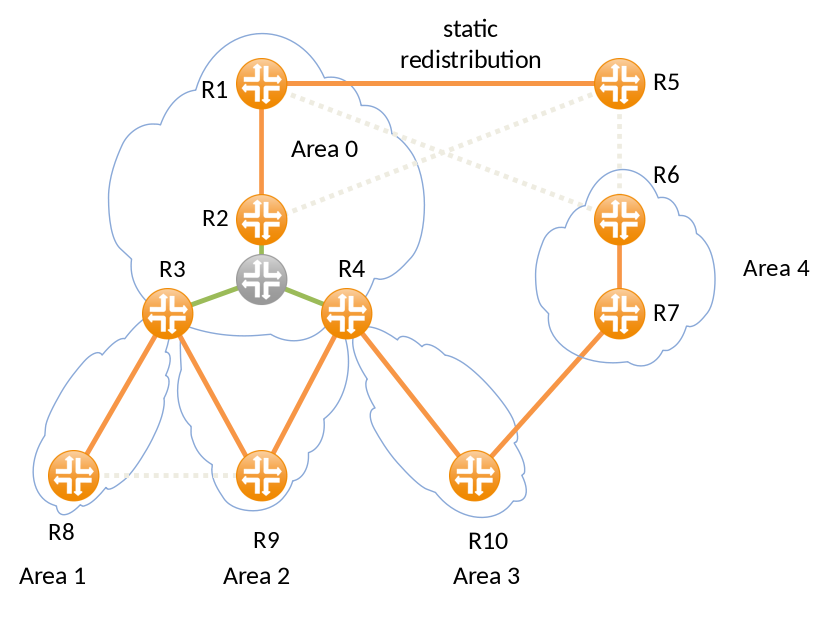
\includegraphics[width=12cm,keepaspectratio]{multiarea_ospf_topo}
\caption{Topológia Multi-area OSPF}
\label{fig:multiarea_ospf_topo}
\end{figure}

\subsection*{Úlohy a ich konfigurácia}
\subsubsection*{Základná konfigurácia}
\subparagraph{Popis}
\subparagraph{}
Ako za základnú konfiguráciu považujeme nastavenie adresácie, vzdialeného prístupu a vypisovania konzoly.
\subparagraph{Konfigurácia}
\noindent
{\fontfamily{qcr}\selectfont
\begin{small}
\begin{verbatim}
!!!!!!!!!!   R1   !!!!!!!!!!
hostname R1
no ip domain-lookup
username admin privilege 15 secret admin
line con 0
	login local
	logging synchronous
line vty 0 15
	privilege level 15
	no login
int lo1
	ip address 10.255.255.1 255.255.255.255
	no shutdown
int f0/1
	ip address 10.100.15.1 255.255.255.0
	no shutdown
int f0/0
	ip address 10.0.12.1 255.255.255.0
	no shutdown

do show ip interface brief


!!!!!!!!!!   R2   !!!!!!!!!!
hostname R2
no ip domain-lookup
username admin privilege 15 secret admin
line con 0
	login local
	logging synchronous
line vty 0 15
	privilege level 15
	no login
int lo1
	ip address 10.255.255.2 255.255.255.255
	no shutdown
int f0/1
	ip address 10.0.234.2 255.255.255.0
	no shutdown
int f0/0
	ip address 10.0.12.2 255.255.255.0
	no shutdown

do show ip interface brief


!!!!!!!!!!   R3   !!!!!!!!!!
hostname R3
no ip domain-lookup
username admin privilege 15 secret admin
line con 0
	login local
	logging synchronous
line vty 0 15
	privilege level 15
	no login
int lo1
	ip address 10.255.255.3 255.255.255.255
	no shutdown
int f0/1
	ip address 10.0.234.3 255.255.255.0
	no shutdown
int f0/0
	ip address 10.1.38.1 255.255.255.0
	no shutdown
int s1/0
	ip address 10.2.39.1 255.255.255.252
	no shutdown

do show ip interface brief


!!!!!!!!!!   R4   !!!!!!!!!!
hostname R4
no ip domain-lookup
username admin privilege 15 secret admin
line con 0
	login local
	logging synchronous
line vty 0 15
	privilege level 15
	no login
int lo1
	ip address 10.255.255.4 255.255.255.255
	no shutdown
int f0/1
	ip address 10.0.234.4 255.255.255.0
	no shutdown
int f0/0
	ip address 10.2.49.1 255.255.255.0
	no shutdown
int s1/0
	ip address 10.3.104.1 255.255.255.252
	no shutdown

do show ip interface brief


!!!!!!!!!!   R5   !!!!!!!!!!
hostname R5
no ip domain-lookup
username admin privilege 15 secret admin
line con 0
	login local
	logging synchronous
line vty 0 15
	privilege level 15
	no login
int lo1
	ip address 10.255.255.5 255.255.255.255
	no shutdown
int f0/1
	ip address 10.100.15.2 255.255.255.0
	no shutdown

do show ip interface brief

!!!!!!!!!!   R6   !!!!!!!!!!
hostname R6
no ip domain lookup
username admin privil 15 secret admin
line con 0
	login local
	logging synchro
line vty 0 15
	privilege level 15	
	no login
int lo1
	ip add 10.255.255.6 255.255.255.255
	no sh
int fa0/1 
	ip add 10.4.67.1 255.255.255.0
	no sh

!!!!!!!!!!   R7   !!!!!!!!!!
hostname R7
no ip domain lookup
username admin privil 15 secret admin
line con 0
	login local
	logging synchro
line vty 0 15
	privilege level 15	
	no login
int lo1
	ip add 10.255.255.7 255.255.255.255
	no sh
int fa0/1 
	ip add 10.4.67.2 255.255.255.0
	no sh
int s1/1
	ip add 10.4.107.1 255.255.255.0
	no sh

!!!!!!!!!!   R8   !!!!!!!!!!
hostname R8
no ip domain lookup
username admin privil 15 secret admin
line con 0
	login local
	logging synchro
line vty 0 15
	privilege level 15	
	no login
int lo1
	ip add 10.255.255.8 255.255.255.255
	no sh
int fa0/0 
	ip add 10.1.38.2 255.255.255.0
	no sh

!!!!!!!!!!   R9   !!!!!!!!!!
hostname R9
no ip domain lookup
username admin privil 15 secret admin
line con 0
	login local
	logging synchro
line vty 0 15
	privilege level 15	
	no login
int lo1
	ip add 10.255.255.9 255.255.255.255
	no sh
int fa0/0 
	ip add 10.2.49.2 255.255.255.0
	no sh
int s1/0
	ip add 10.2.39.2 255.255.255.0
	no sh

!!!!!!!!!!   R10   !!!!!!!!!!
hostname R10
no ip domain lookup
username admin privil 15 secret admin
line con 0
	login local
	logging synchro
line vty 0 15
	privilege level 15	
	no login
int lo1
	ip add 10.255.255.10 255.255.255.255
	no sh
int s1/1 
	ip add 10.4.107.2 255.255.255.0
	no sh
int s1/0
	ip add 10.3.104.2 255.255.255.0
	no sh
\end{verbatim}

\end{small}

}
\subparagraph{Overenie}
\subparagraph{}
Základnú konfiguráciu sme overili príkazmi:\\
\\
\noindent
show ip interface brief

\noindent
{\fontfamily{qcr}\selectfont
\begin{small}
\begin{verbatim}
výpis

\end{verbatim}
\end{small}
}

\noindent
\\
show cdp neighbors

\noindent
{\fontfamily{qcr}\selectfont
\begin{small}
\begin{verbatim}
výpis

\end{verbatim}
\end{small}
}


\subsubsection*{Nakonfigurovať OSPF s viacerými oblasťami}
\subparagraph{Popis}
\subparagraph{}
Jednotlivé smerovače sme priradili do oblastí podľa obrázku \ref{fig:multiarea_ospf_topo}.

\subparagraph{Konfigurácia}
\noindent
{\fontfamily{qcr}\selectfont

% Urob text mensi, aby sa vosiel na sirku obrazovky
\begin{small}

% Pouzijeme "verbatim", aby sme escapeovali cely odsek
\begin{verbatim}
!KONFIGURACIA R1
router ospf 1
    network 10.255.255.1 0.0.0.0 area 0
    exit
int f0/0
    ip ospf 1 area 0
    !treba zapnut interface, ked nam padne router/server
    no shutdown

!KONFIGURACIA R2
router ospf 1
    network 10.255.255.2 0.0.0.0 area 0
    exit
int f0/0
    ip ospf 1 area 0
    no shutdown
int f0/1
    ip ospf 1 area 0
    no shutdown

!KONFIGURACIA R3
router ospf 1
    network 10.255.255.3 0.0.0.0 area 1
    exit
int f0/1
    ip ospf 1 area 0
    no shutdown
int f0/0
    ip ospf 1 area 1
    no shutdown
int s1/0
    ip ospf 1 area 2
    no shutdown

!KONFIGURACIA R4
router ospf 1
    network 10.255.255.4 0.0.0.0 area 3
    exit
int f0/1
    ip ospf 1 area 0
    no shutdown
int f0/0
    ip ospf 1 area 2
    no shutdown
int s1/0
    ip ospf 1 area 3
    no shutdown


!KONFIGURACIA R5
ip route 0.0.0.0 0.0.0.0 f0/1 10.100.15.1

!KONFIGURACIA R6
router ospf 1
    network 10.255.255.6 0.0.0.0 area 4
    exit
int f0/1
    ip ospf 1 area 4
    no sh

!KONFIGURACIA R7
router ospf 1
    network 10.255.255.7 0.0.0.0 area 4
    exit
int f0/1
    ip ospf 1 area 4
    no sh
int s1/1
    ip ospf 1 area 4
    no sh

!KONFIGURACIA R8
router ospf 1
    network 10.255.255.8 0.0.0.0 area 1
    exit
int f0/0
    ip ospf 1 area 1
    no sh

!KONFIGURACIA R9
router ospf 1
    network 10.255.255.9 0.0.0.0 area 2
    exit
int f0/0
    ip ospf 1 area 2
    no sh
int s1/0
    ip ospf 1 area 2
    no sh 

!KONFIGURACIA R10
router ospf 1
    network 10.255.255.10 0.0.0.0 area 3
    exit
int s1/0
    ip ospf 1 area 3
    no sh
int s1/1
    ip ospf 1 area 4
    no sh
\end{verbatim}

\end{small}

}

\subparagraph{Overenie}
\subparagraph{}
Príslušnosť smerovačov do oblastí sme testovali týmito príkazmi:\\
\\
\noindent
show ip ospf interface brief

\noindent
{\fontfamily{qcr}\selectfont
\begin{small}
\begin{verbatim}
výpis

\end{verbatim}
\end{small}
}

\noindent
\\
show ip ospf neighbors

\noindent
{\fontfamily{qcr}\selectfont
\begin{small}
\begin{verbatim}
výpis

\end{verbatim}
\end{small}
}



\subsubsection*{R2, R3, R4 broadcast spojenia prostredníctvom L2 prepínača, zvyšok spojení P2P}
\subparagraph{Popis}
\subparagraph{}

\subparagraph{Konfigurácia}
\noindent
{\fontfamily{qcr}\selectfont

% Urob text mensi, aby sa vosiel na sirku obrazovky
\begin{small}

% Pouzijeme "verbatim", aby sme escapeovali cely odsek
\begin{verbatim}
!KONFIGURACIA R1
int f0/0
    ip ospf network point-to-point

!KONFIGURACIA R2
int f0/0
    ip ospf network point-to-point

!KONFIGURACIA R3
int f0/0
    ip ospf network point-to-point
int s1/0
    ip ospf network point-to-point

!KONFIGURACIA R4
int f0/0
    ip ospf network point-to-point
int s1/0
    ip ospf network point-to-point

!KONFIGURACIA R6
int f0/1
    ip ospf network point-to-point

!KONFIGURACIA R7
int f0/1
    ip ospf network point-to-point
int s1/1
    ip ospf network point-to-point

!KONFIGURACIA R8
int f0/0
    ip ospf network point-to-point

!KONFIGURACIA R9
int f0/0
    ip ospf network point-to-point
    ip ospf 1 area 2
int s1/0
    ip ospf network point-to-point

!KONFIGURACIA R10
int s1/0
    ip ospf network point-to-point
int s1/1
    ip ospf network point-to-point
\end{verbatim}

\end{small}

}

\subparagraph{Overenie}
\subparagraph{}



\subsubsection*{Router-id - loopback0, passive-interface}
\subparagraph{Popis}
\subparagraph{}

\subparagraph{Konfigurácia}
Na každom routri sme vykonali tieti príkazy:
\noindent
{\fontfamily{qcr}\selectfont

% Urob text mensi, aby sa vosiel na sirku obrazovky
\begin{small}

% Pouzijeme "verbatim", aby sme escapeovali cely odsek
\begin{verbatim}
router ospf 1
    router-id 10.255.255.X
    passive-interface lo1
\end{verbatim}

\end{small}

}


'X' symbolizuje číslo smerovača (napr. pre R1: 10.255.255.1)

\subparagraph{Overenie}
\subparagraph{}



\subsubsection*{Area 1 – Totally Stubby}
\subparagraph{Popis}
\subparagraph{}

\subparagraph{Konfigurácia}

\subparagraph{Overenie}
\subparagraph{}



\subsubsection*{Area 3 – Stub}
\subparagraph{Popis}
\subparagraph{}

\subparagraph{Konfigurácia}

\subparagraph{Overenie}
\subparagraph{}



\subsubsection*{Area 4 – pripojenie pomocou virtuálnej linky}
\subparagraph{Popis}
\subparagraph{}

\subparagraph{Konfigurácia}

\subparagraph{Overenie}
\subparagraph{}



\subsubsection*{Statická redistribúcia smerovacích záznamov z R5}
\subparagraph{Popis}
\subparagraph{}
Na smerovači R5 sme nastavili predvolenú cestu.

\subparagraph{Konfigurácia}
\noindent
{\fontfamily{qcr}\selectfont
\begin{small}
\begin{verbatim}

ip route 0.0.0.0 0.0.0.0 f0/1 10.100.15.1

\end{verbatim}
\end{small}
}

\paragraph{}
Potom sme na smerovači R1 namapovali cestu k "lo1" na R5, ktorú sme ohlásili v rámci OSPF topológie príkazmi "redistribute":

\noindent
{\fontfamily{qcr}\selectfont
\begin{small}
\begin{verbatim}

ip route 10.255.255.5 255.255.255.255 f0/1 10.100.15.2
router ospf 1
    redistribute static subnets
    redistribute connected subnets

\end{verbatim}
\end{small}
}

\subparagraph{Overenie}
\subparagraph{}

\noindent
show ip route



\subsubsection*{Kontrola DR prostredníctvom  “ip ospf priority”}
\subparagraph{Popis}
\subparagraph{}
Smerovač R4 sme manuálne nastavili ako DR.

\subparagraph{Konfigurácia}
\noindent
{\fontfamily{qcr}\selectfont
\begin{small}
\begin{verbatim}

int f0/1
    ip ospf priority 100

\end{verbatim}
\end{small}
}

\subparagraph{Overenie}
\subparagraph{}




\subsubsection*{Kontrola OSPF databáz a smerovacích tabuliek}
\subparagraph{Popis}
\subparagraph{}

\subparagraph{Konfigurácia}

\subparagraph{Overenie}
\subparagraph{}




\subsubsection*{Kontrola konektivity}
\subparagraph{Popis}
\subparagraph{}
Konektivitu sme testovali pomocou tclsh skriptu.

\subparagraph{Konfigurácia}

\subparagraph{Overenie}
\subparagraph{}


\subsubsection*{Area 2 – R3 primárny smerovač, R4 sekundárny smerovač so sumarizovanými internými smerovacími záznamami do jedného sumarizačného}
\subparagraph{Popis}
\subparagraph{}
Smerovač R3 sme nastavili ako primárneho a R4 ako sekundárny smerovač.

\subparagraph{Konfigurácia}
\noindent
{\fontfamily{qcr}\selectfont
\begin{small}
\begin{verbatim}

int f0/0
    bandwidth 1

\end{verbatim}
\end{small}
}

\subparagraph{}
Tým, že znížime bandwidth na tomto rozhraní, zvýšime jeho "Cost". Zmena sa potom ohlási všetkým smerovačom v sieti. Následkom toho bude rozhranie f0/1 na R3 preferované pre ďalšie smerovanie.

\subparagraph{Overenie}
\subparagraph{}
\noindent
show ip ospf interface f0/1



\subsubsection*{Skrátenie hello a dead-interval časovačov, zistenie funkčnosti vytrhnutím jednej z liniek smerom ku L2 prepínaču}
\subparagraph{Popis}
\subparagraph{}
Smerovačom R2, R3 a R4 sme znížili \say{hello} a \say{dead} intervaly na rozhraniach pripojených k prepínaču.

\subparagraph{Konfigurácia}

\subparagraph{Overenie}
\subparagraph{}
\noindent
show ip ospf interface f0/1

\end{document}
